% chapter1.tex
\chapter{Examples}

\section{Theorem System}

\defn{Definition Name}{
    A definition.
}

\thmr{Theorem Name}{mybigthm}{
    A theorem.
}

\lem{Lemma Name}{
    A lemma.
}

\fact{
    A fact.
}

\cor{
    A corollary.
}

\prop{}{
    A proposition.
}

\exer{
    Exercise example.
}

\clmp{}{
    A claim.
}{
    A reference to Theorem~\ref{thm:mybigthm}
}

\pf{
    Veniam velit incididunt deserunt est proident consectetur non velit ipsum voluptate nulla quis. Ea ullamco consequat non ad amet cupidatat cupidatat aliquip tempor sint ea nisi elit dolore dolore. 

    Laboris labore magna dolore eiusmod ea ex et eiusmod laboris. Et aliquip cupidatat reprehenderit id officia pariatur. 
}

\ex{
    Nostrud esse occaecat Lorem dolore laborum exercitation adipisicing eu sint sunt et. Excepteur voluptate consectetur qui ex amet esse sunt ut nostrud qui proident non. Ipsum nostrud ut elit dolor. Incididunt voluptate esse et est labore cillum proident duis.
}



\rmk{
    Some remark.
}

\rmkb{
    Some more remark.
}

\section{Pictures}

\begin{figure}[H]
    \center
    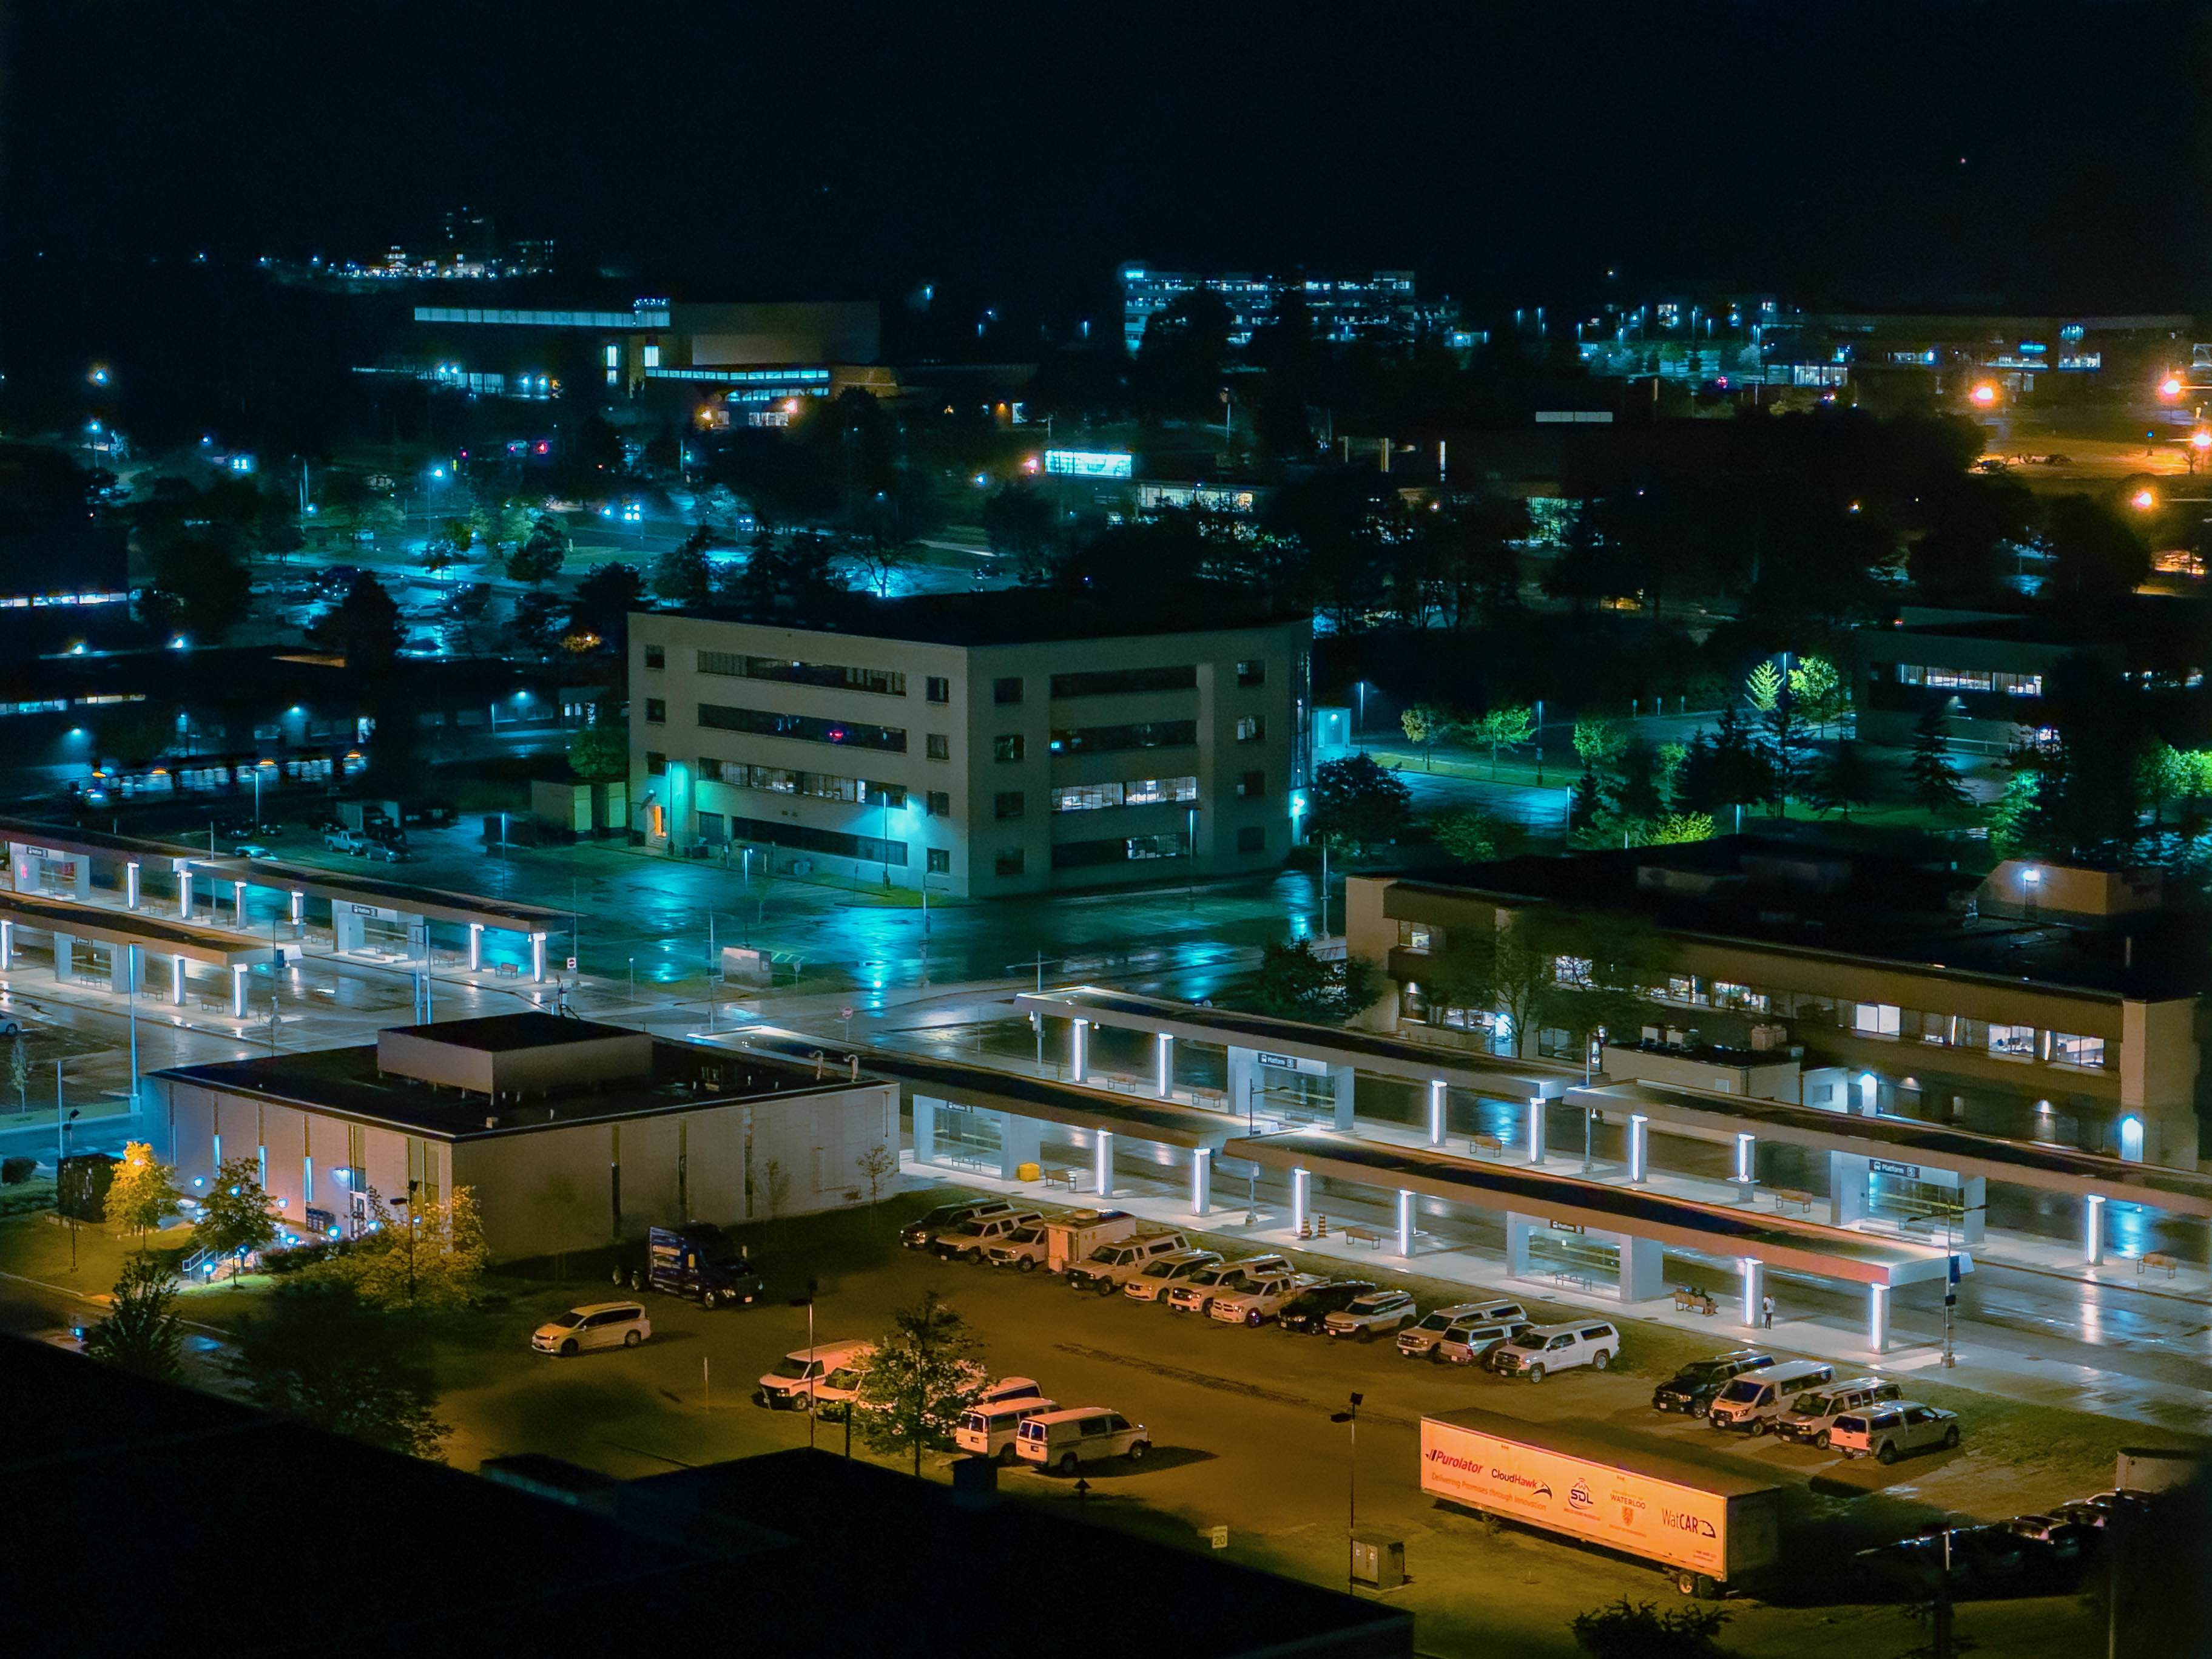
\includegraphics[scale=0.1]{img/loo.jpg}
    \caption{Waterloo, ON}
\end{figure}